\documentclass[10pt,a4paper]{article}
\usepackage[utf8]{inputenc}
\usepackage{amsmath}
\usepackage{gensymb}
\usepackage{amsfonts}
\usepackage{siunitx}
\usepackage[european]{circuitikz}
\usepackage{geometry}
\newgeometry{tmargin=2cm, bmargin=2cm, lmargin=2cm, rmargin=2cm}
\usepackage{amssymb}
\usepackage{polski}
\usepackage{graphicx}
\author{\textbf{T. Fąs}}
\title{\textbf{BADANIE DRGAŃ STRUNY}}
\begin{document}
\maketitle



\begin{center}
\textbf{\subsection*{STRESZCZENIE}}
\end{center}
W eksperymencie udało się potwierdzić modelową zależność między częstotliwością drgania własnego, a liczbą falową. Nie udało się wykazać zgodności w przypadku zależności między częstotliwością drgania własnego, a długością struny oraz między częstotliwością drgania własnego, a siłą naciągu struny. Wyznaczono również prędkość fali $v=310,29\pm0,33$ m/s oraz gęstość struny $\rho=8373\pm334$ kg/m$^3$.

\begin{center}
\textbf{\subsection*{WSTĘP}}
\end{center}
Jeżeli strunę o długości $L$, gęstości $\rho$ i przekroju poprzecznym $S$ rozciągniemy siłą o wartości $F$ i wprawimy w drgania, to jej ruch będzie podlegał równaniu falowemu. Jeśli struna ta jest zaczepiona na obu końcach, to w wyniku drgań powstanie fala stojąca, a częstość drgań tej struny dana jest wzorem:
\begin{equation}
\nu_{n}=\dfrac{n}{2L}v=\dfrac{n}{2L}\sqrt{\dfrac{F}{\rho S}},
\end{equation}
gdzie $v$ jest prędkością fali, a $n$ jest liczbą odpowiadającą kolejnym modom własnym struny. 

Celem ćwiczenia było zbadanie zależności wyrażonej Równaniem (1) dla różnych wartości $n$, $L$ i $F$ oraz wyznaczenie prędkości $v$ i gęstości $\rho $ struny.


\begin{center}
\textbf{\subsection*{UKŁAD DOŚWIADCZALNY}}
\end{center}
Układ składał się z odważników o różnych masach, szalki, stalowej struny, wzmacniacza, oscyloskopu oraz generatora RC jaki i dwóch elektromagnesów: jeden z nich podłączony do generatora RC pobudzał strunę do drgań, a drugi służył jako odbiornik. W pomiarach wykorzystano także śrubę mikrometryczną oraz miarkę. Schemat układu przedstawia Rysunek 1.

\begin{figure}[h!]
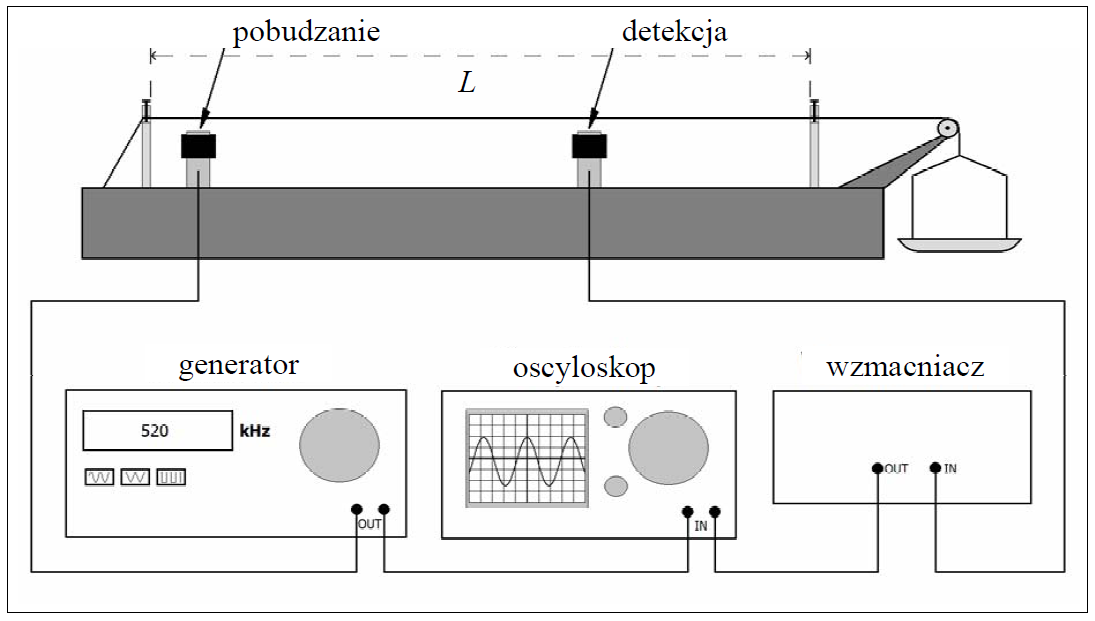
\includegraphics[width=15cm]{rap10rr1} 
\centering
\caption{Schemat układu pomiarowego.}
\end{figure}

Struna była pod działaniem siły naciągu wynikającej z obciążenia szalki. Długość struny kontrolowano, przesuwając jeden z jej punktów zaczepienia. Szukanie modów drgań struny polegało na takim dobraniu częstości drgań na generatorze, aby doszło do zjawiska rezonansu. Pomagał w tym oscyloskop, który rysował funkcję amplitudy. Otrzymanie maksimum amplitudy oznaczało wystąpienie rezonansu.

\begin{center}
\textbf{\subsection*{WYNIKI POMIARÓW}}
\end{center}
Pomiary średnicy struny zostały wykonane przy pomocy śruby mikrometrycznej w różnych miejscach struny. Wyniki pomiarów przedstawia Tabela 1.

\begin{table}[h!]
\centering
\caption{Średnica $D$ struny.}

\begin{tabular}{|c|c|c|c|c|c|c|c|}
\hline
Średnica $D$ {[}mm{]} & 0,29 & 0,30 & 0,30 & 0,30 & 0,30 & 0,30 & 0,30 \\ \hline
\end{tabular}
\end{table}

Następnie dokonano pomiarów długości $L$ struny przy pomocy miarki. Otrzymano $L=76,1$ cm. Dla takiej długości zmierzono częstości własne struny od $n=1$ do $n=6$. W trakcie pomiarów obiekt znajdował się pod obciążeniem 5 kg plus 0,756 kg wynikających z masy szalki. Wyniki pomiarów przedstawia Tabela 2.

\begin{table}[h!]
\centering
\caption{Pomiary częstości struny: stała długość i siła.}
\begin{tabular}{|c|c|c|c|c|c|c|}
\hline
Liczba $n$              & 1       & 2       & 3       & 4       & 5        & 6        \\ \hline
Częstość $\nu_{n}$ [Hz] & 204,685 & 406,500 & 611,260 & 815,551 & 1019,870 & 1223,190 \\ \hline
\end{tabular}
\end{table}

W kolejnym etapie szukano częstości drgań własnych $\left( n=1 \right)$ dla różnych długości struny, przy obciążeniu takim samym jak przy poprzednich pomiarach. Wartości otrzymanych częstości przedstawione są w Tabeli 3. 

\begin{table}[h!]
\centering
\caption{Pomiary częstości struny: różne długości.}
\begin{tabular}{|c|c|c|c|c|c|c|}
\hline
Długość $L$ [cm]        & 76,1    & 70,1    & 66,5    & 64,8    & 62,3    & 60,5    \\ \hline
Częstość $\nu_{n}$ [Hz] & 204,685 & 219,595 & 223,660 & 236,485 & 245,960 & 255,585 \\ \hline
\end{tabular}
\end{table}

Ostatni etap dotyczył szukania częstości podstawowej dla różnych obciążeń struny. Na potrzeby pomiarów powrócono do długości 76,1 cm, a siłę naciągu zmieniano poprzez zmianę obciążników. Wyniki przedstawione są w Tabeli 4.

\begin{table}[h!]
\centering
\caption{Pomiary częstości struny: różne masy.}
\begin{tabular}{|c|c|c|c|c|c|c|}
\hline
Masa obciążnika [kg] & 5       & 4       & 3       & 2       & 1,5     & 1       \\ \hline
Częstość $\nu$ [Hz]  & 204,188 & 183,767 & 163,600 & 140,045 & 126,705 & 118,294 \\ \hline
\end{tabular}
\end{table}




\begin{center}
\textbf{\subsection*{ANALIZA DANYCH}}
\end{center}

W celu wyznaczenia niepewności pomiaru częstości wykonano dodatkowy pomiar przy obciążeniu 5 kg i długości 76,1 cm. Otrzymano wartość $\nu_{k}=201,785$ Hz. Porównano tę wartość z wartością z Tabeli 2 wynoszącą $\nu_{1}=204,685$ Hz i postanowiono przyjąć niepewność pomiaru $u_{\nu}$, jako różnicę $(\nu_{1}-\nu_{k})/2=1,45 $ Hz.

Aby wyznaczyć średnicę struny postanowiono uśrednić wyniki z Tabeli 1 oraz obliczyć odchylenie standardowe średniej, dane wzorem:
\begin{equation}
s^2=\sum_{i=1}^{N}\dfrac{\left(D_{i}-\bar{D}\right)^2}{N(N-1)},
\end{equation}
gdzie $\bar{D}$ jest średnią średnicy, a $N$ jest liczbą pomiarów. Jako, że rozdzielczość śruby mikrometrycznej wynosiła $\Delta=0,01$ mm, to ostateczne niepewność pomiaru średnicy wynosi:
\begin{equation}
u_{D}=\sqrt{s^2+\dfrac{\Delta^2}{3}}
\end{equation}
Ostatecznie otrzymano średnicę $D=0,2986\pm0,0060$ mm.

Dane z Tabeli 2 podlegają Równaniu (1), które można zapisać w sposób:

\begin{equation}
\nu_{n}=an,
\end{equation}
gdzie $a=v/2L$. W ten sposób otrzymano funkcję linową. Aby dopasować dane z Tabeli 2 do Równania (4) zastosowano metodę najmniejszych kwadratów. Polega ona na minimalizacji wielkości, która w tym przypadku dana jest wzorem:
\begin{equation}
R\left(a \right)=\sum_{n=1}^{6}\left(\dfrac{\nu_{n}-an}{u_{\nu}}\right)^2 \quad \cite{tay1}
\end{equation}

Otrzymano wartość $a=203,87\pm0,15$ Hz, przy zastosowaniu niepewności częstości $u_{\nu}=1,45$ Hz. Dane wraz z krzywą najlepszego dopasowania zostały przedstawione na Rysunku 2.

\begin{figure}[h!]
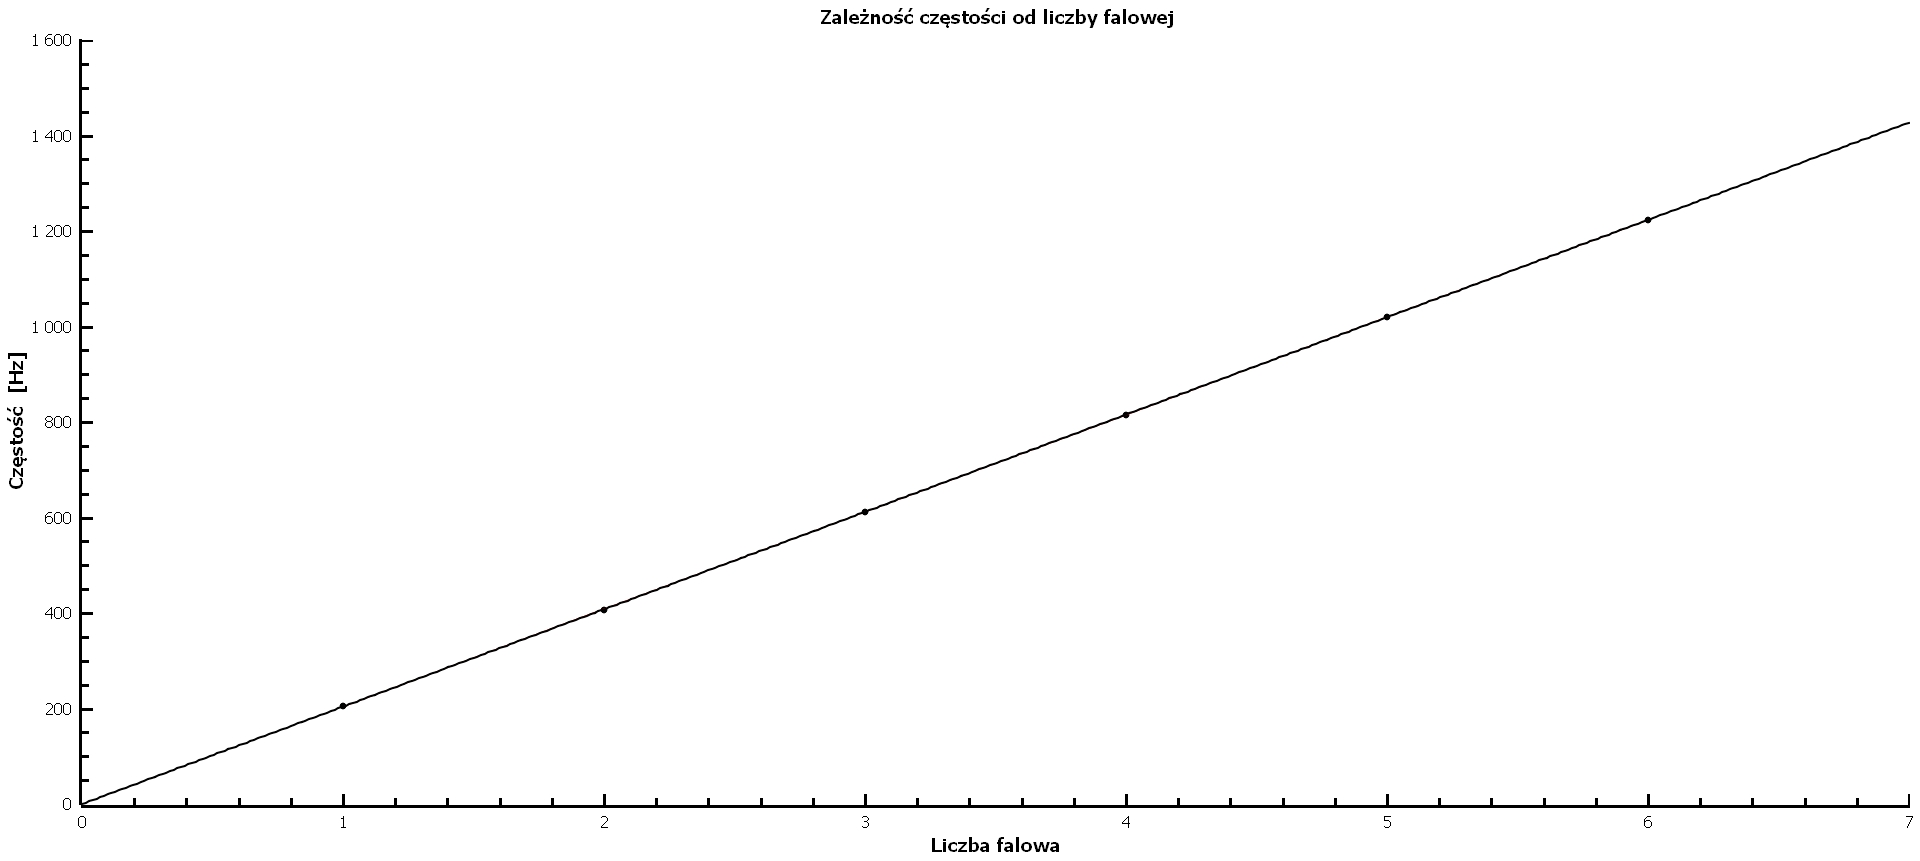
\includegraphics[width=15cm]{rap10rys1} 
\centering
\caption{Krzywa najlepszego dopasowania.}
\end{figure}

Aby zyskać pewność, co do poprawnego dopasowania krzywej, przeprowadzono test $\chi^2$. Polega on na sprawdzeniu, czy wartość $\chi^2$, czyli suma reszt z Równania (5) jest mniejsza od wartości krytycznej $\chi_{0}^2$. Wartość krytyczna zależy od liczby stopni swobody oraz od prawdopodobieństwa popełnienia błędu pierwszego rodzaju. W tym przypadku liczba stopni swobody wynosi 6-1=5, a za prawdopodobieństwo przyjęto wartość $p=0,05$.
Otrzymane wartości wynoszą $\chi^2=1,24$, a $\chi_{0}^2=11,07$. Tak więc otrzymane dane nie są sprzeczne z Równaniem (1). 


Jako, że $a=v/2L$ możliwe jest obliczenie prędkości $v$ fali. Dla wartości $L=76,1$ cm prędkość ta wynosi $v=310,29$ m/s. Niepewność tej wielkości wyznaczono, korzystając z metody propagacji małych błędów. Ogólny wzór przenoszenia niepewności w tej metodzie jest następujący:
 \begin{equation}
 u_{f}^2=\sum_{i=1}^n \left( \dfrac{\partial f}{\partial x_{i}}u_{i}\right)^2+\sum_{i=1, i\neq j}^n \left( \dfrac{\partial f}{\partial x_{i}}\dfrac{\partial f}{\partial x_{j}}c_{ij}\right),
 \end{equation}
 gdzie wielkość $f$ zależy od wielkości $x_{i}$ o niepewnościach $u_{i}$ i o ocenach kowariancji $c_{ij}$ \cite{tay2}. W rozpatrywanym przypadku kowariancja wynosi zero.

Jako, że pomiar długości struny wykonano jednokrotnie, to jej niepewność związana jest tylko i wyłącznie z rozdzielczością miarki, która wynosiła $\Delta_{L}=0,01$ cm. Tak więc ostateczna niepewność długości $L$ wynosi $u_{L}=\Delta_{L}/\sqrt{3}$.
Podstawiając te dane do Równania (6) otrzymano, że niepewność prędkości $v$ wynosi:
\begin{equation}
u_{v}=v\sqrt{\dfrac{u_{a}^2}{a^2}+\dfrac{u_{L}^2}{L^2}}=0,33 \, \dfrac{m}{s}
\end{equation}
Tak więc ostatecznie $v=310,29\pm0,33$ m/s.

Z Równania (1) wynika również, iż $a=n/2L\sqrt{F/\rho S}$. Jako, że siła $F=mg$, gdzie $m$ jest masą ciężarka plus masa szalki, a $S$ można obliczyć, gdyż znana jest średnica $D$ struny, to możliwe jest wyznaczenie gęstości $\rho$ struny.

Masy ciężarków i szalki uznano za znane dokładnie oraz przyjęto $g=9,80665$ m/s$^2$. 

Niepewność przekroju $S=\pi D^2/4$ dana jest, na mocy Równania (6), wzorem:
\begin{equation}
u_{S}=\dfrac{\pi D u_{D}}{2}
\end{equation}
Z kolei niepewność gęstości $\rho=mg/4L^2a^2S$ dana jest wzorem:
\begin{equation}
u_{\rho}=\rho \sqrt{\dfrac{4u_{a}^2}{a^2}+\dfrac{4u_{L}^2}{l^2}+\dfrac{u_{S}^2}{S^2}}
\end{equation}
Podstawienie danych liczbowych zwraca wartość $\rho=8373\pm334$ kg/m$^3$.

Analiza danych z Tabeli 3 również polegała na dopasowaniu krzywej do punktów pomiarowych. 
Tym razem zależność byłą funkcją postaci:
\begin{equation}
\nu=\dfrac{a}{2L},
\end{equation}
gdzie $a=v=\sqrt{F/\rho S}$. W tym przypadku, w celu dopasowania krzywej, skorzystano z programu \textit{gnuplot}. W pierwszej kolejności próbowano przeprowadzić analizę przy pomocy programu \textit{SciDAVis}, jednakże z nieznanych powodów program ten nie był w stanie narysować krzywej dopasowania, pomimo obliczonych parametrów. 

Wyniki otrzymane w \textit{gnuplot} to: $a=306,4\pm1,9$ m/s, $\chi^2=12,63$, a samą krzywą z punktami przedstawiono na Rysunku 3.

\begin{figure}[h!]
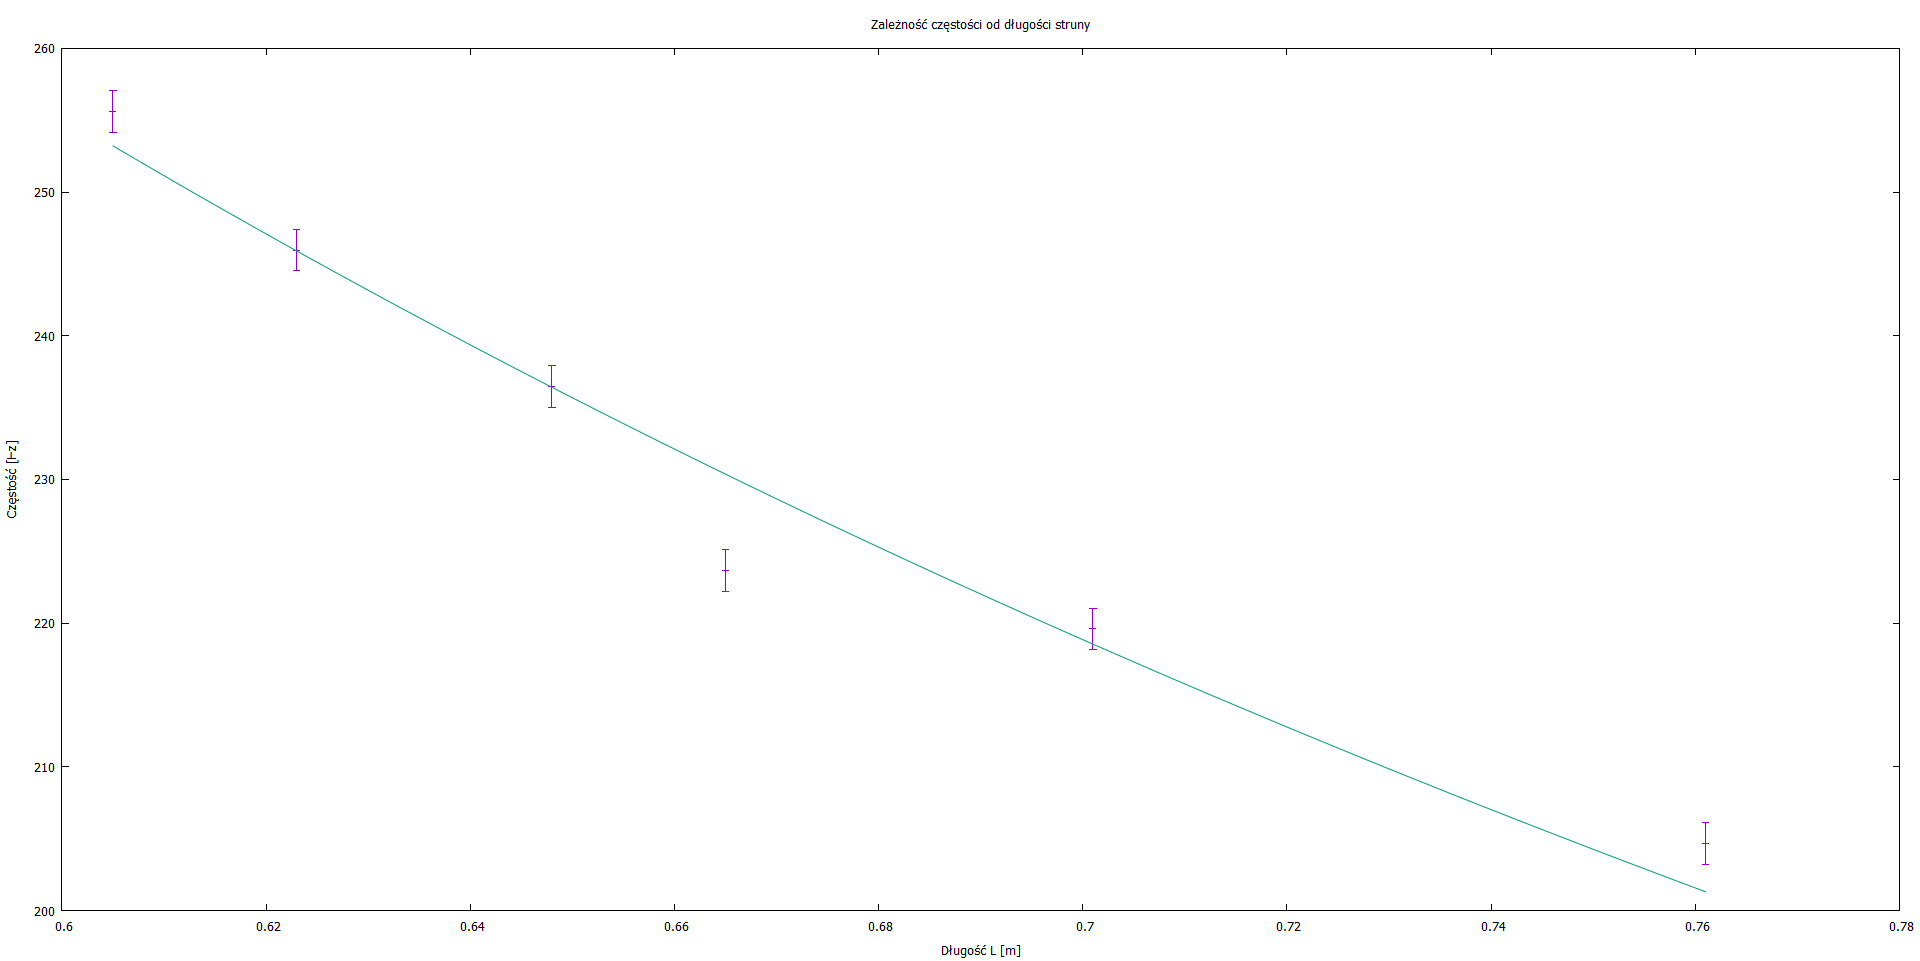
\includegraphics[width=15cm]{rap10rys2} 
\centering
\caption{Krzywa najlepszego dopasowania.}
\end{figure}

Wartość gęstości obliczona z tych danych wynosi $\rho=8588\pm359$ km/m$^3$.

 Niestety, wartość $\chi^2$ jest większa od wartości krytycznej $\chi_{0}^2=11,07$, tak więc dane nie są zgodne z hipotezą, przeczą one Równaniu (10). Z tego też powodu nie można otrzymanych wyników prędkości fali i gęstości porównać z wynikami wcześniejszymi. 

Analogiczną analizę przeprowadzono dla danych z Tabeli 4. W tym przypadku zastosowano zamianę zmiennej: $w=\sqrt{m}$, co prowadzi do funkcji liniowej:
\begin{equation}
\nu=\dfrac{w}{2L}\sqrt{\dfrac{g}{\rho S}}=\alpha w.
\end{equation}
Przy czym przez $m$ rozumie się masę szalki plus obciążenie, a $\alpha=1/2L\sqrt{g/\rho S}$. Wzór wykorzystany w metodzie najmniejszych kwadratów przyjmuje postać analogiczną do Równania (5). Przeprowadzone obliczenia zwracają wynik: $\alpha=84,96\pm0,32$ 1/s$\sqrt{kg}$. Krzywą dopasowania przedstawiono na Rysunku 4. Wyznaczona wartość gęstości wynosi $\rho=8376\pm340$ kg/m$^3$.


\begin{figure}[h!]
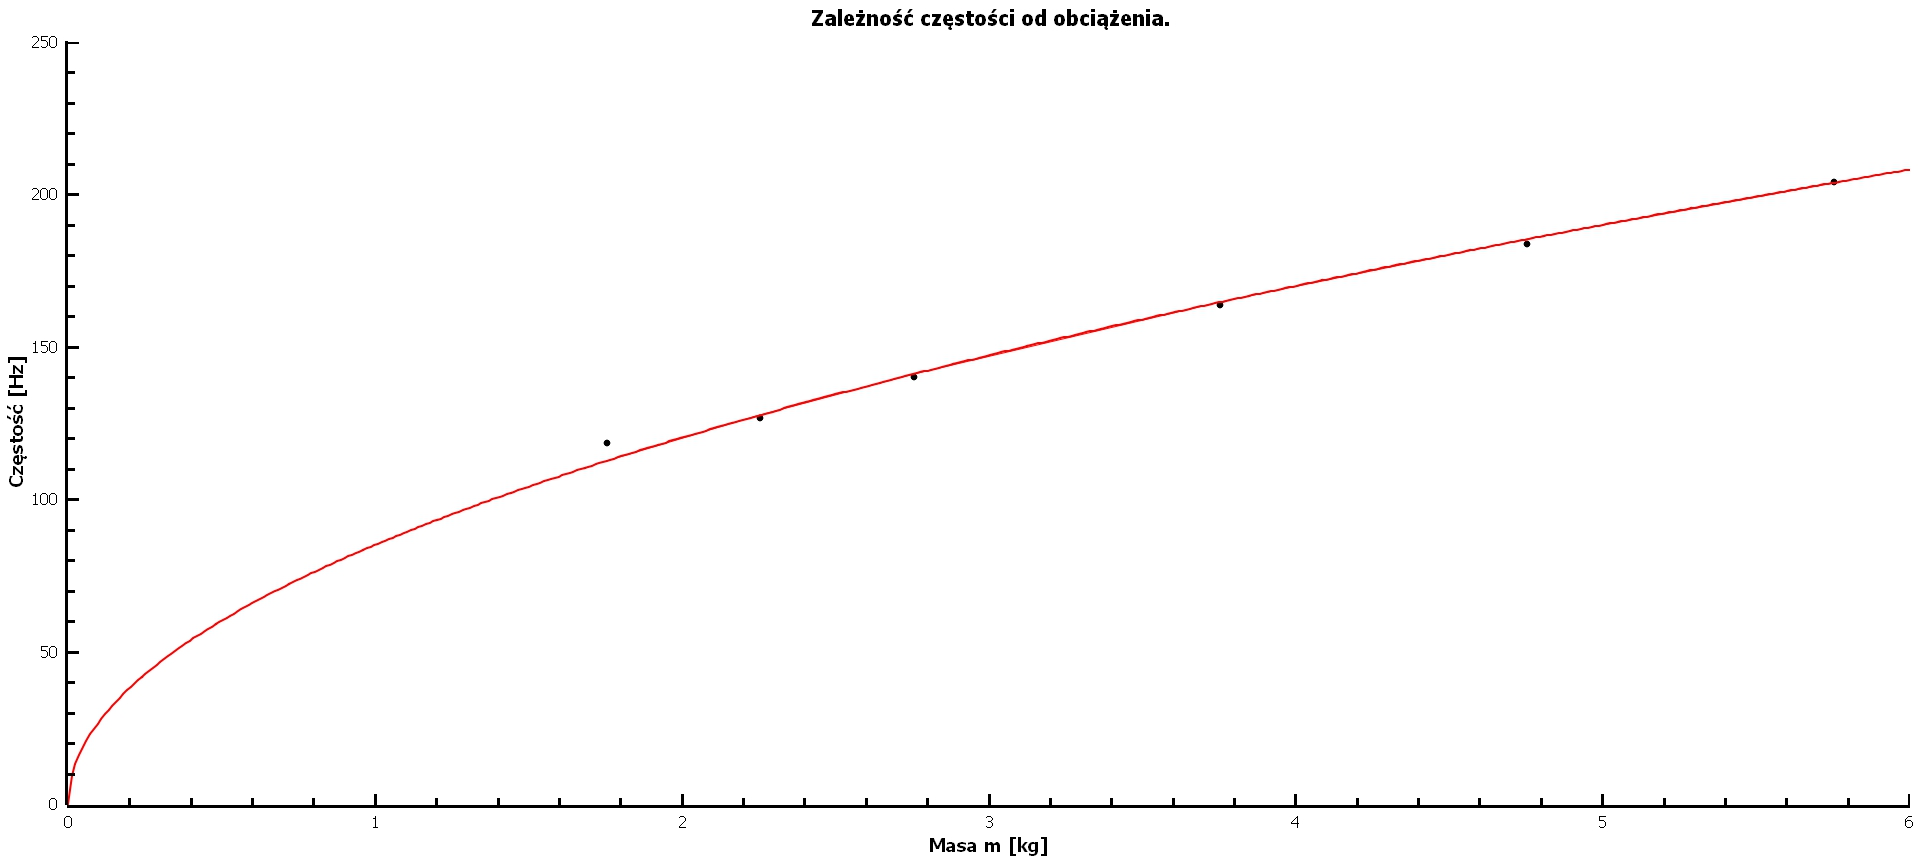
\includegraphics[width=15cm]{rap10rys3} 
\centering
\caption{Krzywa najlepszego dopasowania.}
\end{figure}

Jednakże wartość $\chi^2=18,05$ nie pozwala uznać danych za zgodne z hipotezą. Zarówno tu, jak i w poprzedniej analizie otrzymano wyniki niezgodne z hipotezą. Odrzucenie punktów wyraźnie odstających od krzywej pozwoliłoby uzyskać zgodność, jednakże brakuje wyraźnych powodów odrzucenia tych wyników, szczególnie w przypadku Rysunku 4 odchylenie pierwszego punktu nie jest szczególnie duże. 

\begin{center}
\textbf{\subsection*{DYSKUSJA WYNIKÓW I WNIOSKI}}
\end{center} 

Otrzymane wyniki w większości przypadków nie potwierdzają słuszności Równania (1). Jednakże wziąwszy pod uwagę fakt, że pomiary przeprowadzone w identycznych warunkach mogły zwrócić zupełnie inne wyniki pozwala stwierdzić, iż nie należy przykładać wielkiej wagi do otrzymanych wartości. Ponowienie pomiarów, przy zachowaniu powtarzalności wyników, pozwoliłoby rozstrzygnąć tę kwestię. Dodatkowo na niepewności miał duży wpływ obserwator, który to ostatecznie rozstrzygał o zaistnieniu rezonansu. Zautomatyzowanie tego procesu pozwoliłoby uzyskać dokładniejsze i bardziej powtarzalne wyniki.




\begin{center}
\begin{thebibliography}{9}

 \bibitem{tay1}
 J. R. Taylor,
 \emph{Wstęp do analizy błędu pomiarowego},
 PWN, Warszawa, 1995, s. 175.
 
 
 \bibitem{tay2}
 J. R. Taylor,
 \emph{Wstęp do analizy błędu pomiarowego},
 PWN, Warszawa, 1995, s. 197.
 
\end{thebibliography}

\end{center}


\end{document}